\documentclass[a4paper,10pt]{article}
\usepackage[utf8]{inputenc}
\usepackage[T1]{fontenc}
\usepackage[french]{babel}
\usepackage{textcomp}
\usepackage{listings}
\usepackage{pdfpages}
\usepackage{array}
\usepackage{titling}
\usepackage{geometry}

\geometry{hmargin=2.5cm,vmargin=1.5cm}
\setlength{\hoffset}{-18pt}        
\setlength{\oddsidemargin}{0pt} % Marge gauche sur pages impaires
\setlength{\evensidemargin}{9pt} % Marge gauche sur pages paires
\setlength{\marginparwidth}{54pt} % Largeur de note dans la marge
\setlength{\textwidth}{481pt} % Largeur de la zone de texte (17cm)
\setlength{\marginparsep}{2pt} % Séparation de la marge
\setlength{\topmargin}{0pt} % Pas de marge en haut
\setlength{\headheight}{6pt} % Haut de page
\setlength{\headsep}{10pt} % Entre le haut de page et le texte
\setlength{\footskip}{27pt} % Bas de page + séparation
\setlength{\textheight}{708pt} % Hauteur de la zone de texte (25cm)

\setlength{\droptitle}{-4cm}
\title{Synthèse - Machine Learning}
\author{Léa Calem - Fatima Layla - Laureline Martin}

\begin{document}

\maketitle
	
\section{Description du jeu de données}
	\subsection{Les données}
	% \subsubsection{Modélisation des données sous forme de matrice}
		Nous disposons de 14 000 images représentant soit des t-shirts/tops, soit des robes. La classe $C_1 =$ \{0 T-shirt/top\} et la classe $C_2 =$ \{3 Dress\}.
		\begin{itemize}
			\item 7 000 images de la classe $C_1$
			\item 7 000 images de la classe $C_2$
		\end{itemize}
		Les images de taille 28x28 pixels (784 pixels) composées de niveau de gris (valeur allant de 0 à 255). Sur ces images, seul l’objet est coloré donc le reste de l’image est en blanc, la valeur des pixels à 0.\\
		Ces images sont issues des classes 0 et 3 du jeu données Fashion-MNIST (http://www.openml.org/d/40996). 
	\subsection{Séparation des jeux de données}
		\begin{enumerate}
			\item Données d’entraînement : sous-ensemble de données destiné à l’apprentissage du modèle. Nous utilisons 80\% des données pour l'apprentissage, soit 11 200 images.
			\item Données de test : sous-ensemble de données destiné à l’évaluation du modèle (ce jeu de données ne doit en aucun cas être utilisé lors de la conception du modèle). Nous utilisons 20\% des données, soit 2 800 images.
		\end{enumerate}

	\subsection{Description statistique}
		Ci-dessous, un graphe représente un échantillon de 200 images (108 de la classe $C_1$ et 92 de $C_2$) avec en ordonné le rapport décrit ci-dessus et en abscisse le numéro de l'image. 
		\begin{itemize}
			\item Bleu : classe $C_1$
			\item Orange : classe $C_2$
		\end{itemize}
		Nous avons divisé l’image en 3 tiers horizontaux, puis nous calculons la moyenne du blanc de la 1ère et 3éme partie. Les t-shirts ont une moyenne de blanc moins importante sur le 1er tiers de l'image que sur le 3e tiers (car les manches sont plus larges que le reste du tissu), tandis que les moyennes de blanc pour les robes sont similaires pour le 1er et le 3e tiers de l'image (manches et la jupe du vêtement prennent autant d'espace sur l'image). On considère que les pixels inférieurs à 25 sont blancs.\\

		%images
		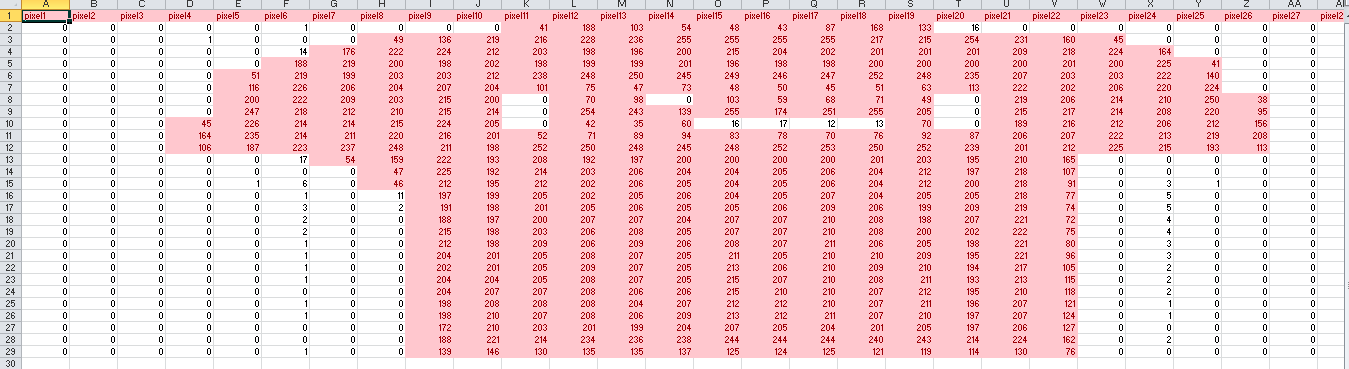
\includegraphics[scale = 0.25]{fichiers/ex_tshirt.PNG}
		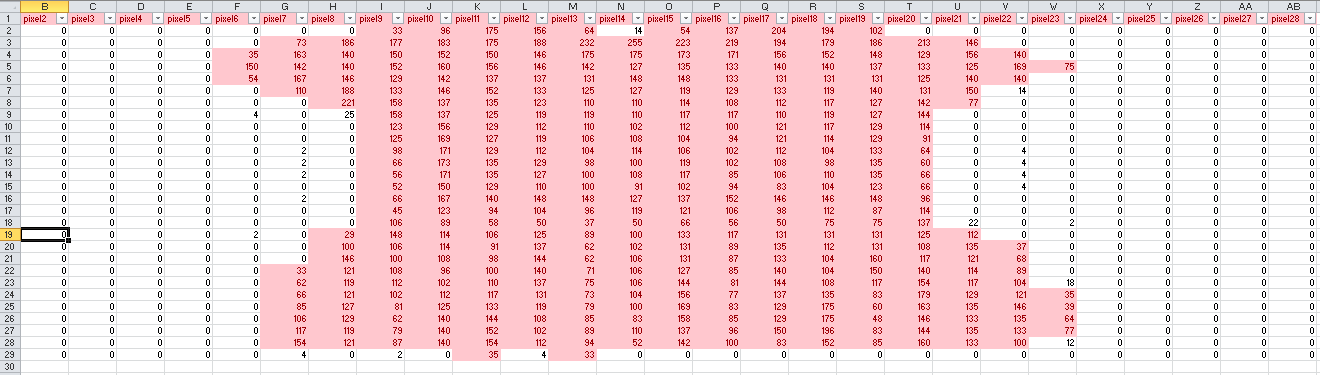
\includegraphics[scale = 0.25]{fichiers/ex_robe.PNG}
		\vfill\begin{center} 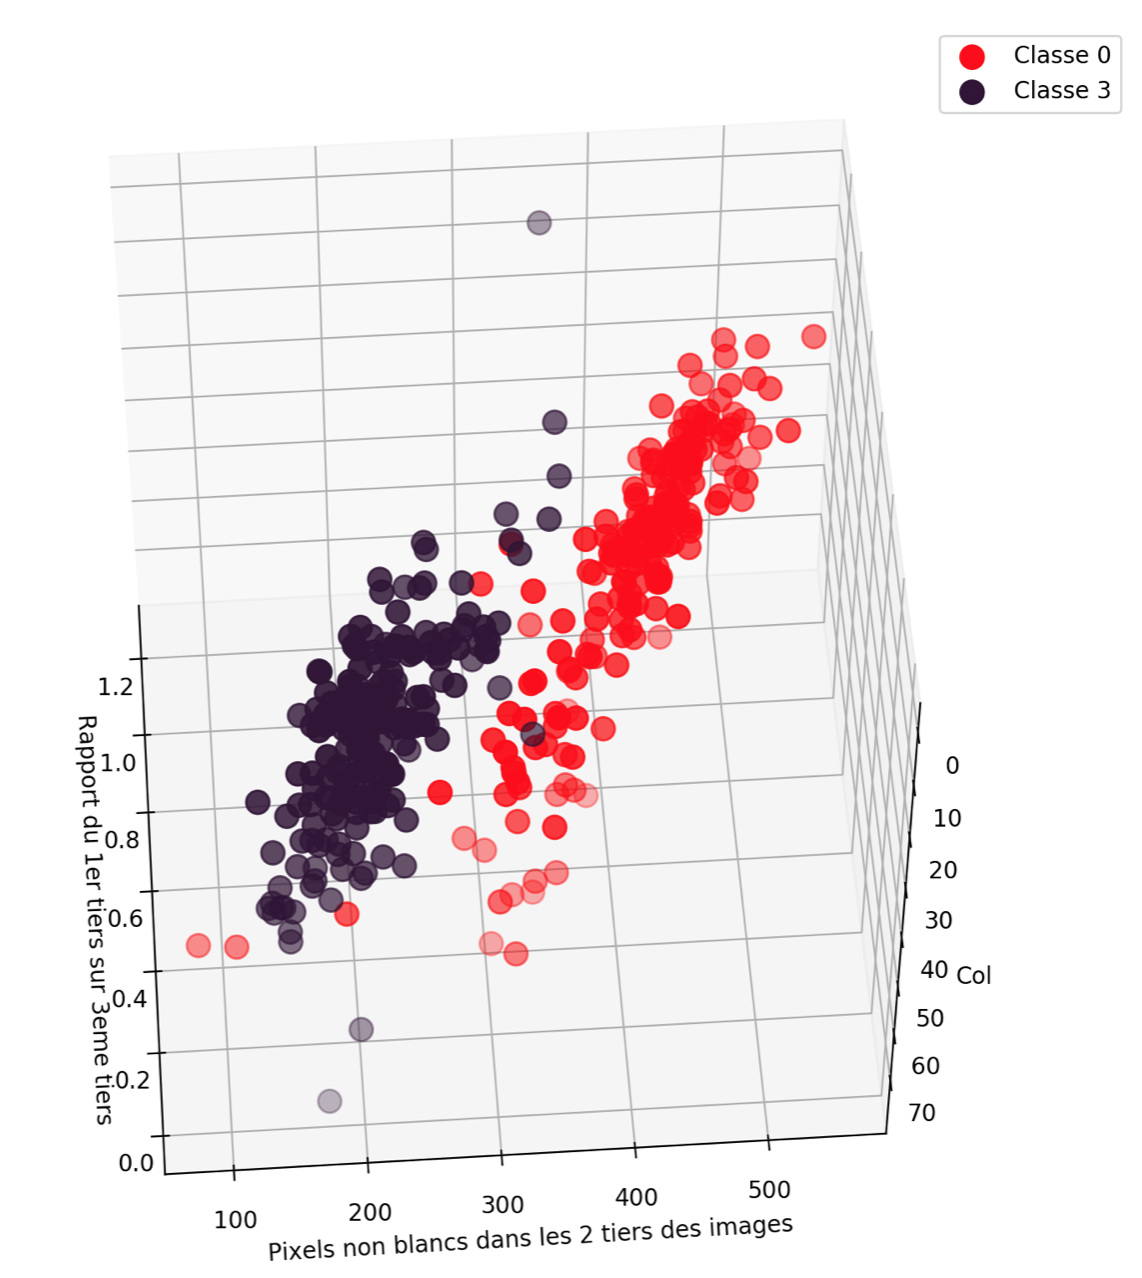
\includegraphics[scale = 0.6]{fichiers/rapport.PNG} \end{center}\vfill
		


\newpage
\section{Méthodologie}
	\subsection{Méthodologie générale}
		Dans ce projet, nous allons classifier des images en deux catégories : t-shirts/tops ou robes.\\
		Les méthodes d'apprentissages que nous allons utiliser sont de type supervisées car nos données sont déjà annotées :
		$$ S = {(x_i, y_i)} $$
		Tel que : $x_i$ = ième image de l'ensemble des images, $y_i$ = ième étiquette de l'ensemble des étiquettes des classes $C_1$ et $C_2$.\\
		% Classification : $y_i = {C_1, C_2}$.
		Avec les classes : $C_1 =$ \{0 T-shirt/top\} et $C_2 =$ \{3 Dress\}.\\
		\\
		Nous allons utiliser plusieurs méthodes d’apprentissage qui vont nous permettre de définir la fonction d'appprentissage $h(x)$ telle que : $h(x) = (\hat y)$. Ainsi, nous obtiendrons des valeurs $(\hat y)_i$ proches des $y_i$, pour tout $(x_i, y_i)$ appartenant à $S$.\\
		%(cours 02\_methodo\_etu.pdf/ slide 9)

	\subsection{Paramètres}
		Comme les images $x_i$ sont bruitées, nous supposons que les pixels ayant une valeur < 25 sont blancs.
		Pour trouver ce seuil, nous avons testé plusieurs valeurs de pixels : 15, 25 et 35 et nous en avons conclu que 25 était la plus adéquat pour définir la valeur bruitée avec le minimum d'erreur (confusion avec l'objet).\\
		Nous évaluons comme paramètre le nombre de pixels blancs du premier tiers de l'image (horizontal) par rapport au troisième tiers. Comme le vêtement est symétrique, ce rapport se fait sur la moitié gauche de l'image. Ainsi, \\
		Néanmoins, on remarque que sur 2 dimensions les classes se superposent encore dû aux tops et aux robes qui ont des rapports proches. Nous allons donc augmenter cet espace d'une dimension en calculant le rapport des pixels blancs entre le deuxième tiers et le troisième tiers. Les robes ayant une jupe évasée contrairement aux tops. \\
		Notre espace est donc le suivant :
		\begin{itemize}
			\item Pour l'axe $x$ : N° objet
			\item Pour l'axe $y$ : rapport 1er tiers/ 3e tiers
			\item Pour l'axe $z$ : rapport 2e tiers / 3e tiers
		\end{itemize}
		Nous évaluons pour les axes $y$ et $z$ les rapports de deux surfaces de 9x9 pixels tel que : \\
		Graphiquement :
		$$ \forall pixels_{i,j} < 25,  (\sum_{i=1} ^9 \sum_{j=1} ^9  (pixels_{i,j})) / (\sum_{i=19} ^{28} \sum_{j=1}^9  (pixels_{i,j}) ) $$
		Pour le jeu de données :
		$$ \forall pixels_j < 25, (\sum_{i=0} ^8 \sum_{j=1} ^9  (pixels_j +28i) ) / (\sum_{i=18} ^{27} \sum_{j=1} ^9  (pixels_j+28i) ) $$
		(pour le calcul de l'axe $z$ on remplace les bornes des sommes du numérateur par $i=10$ à 19).

	\subsection{Méthodes d'apprentissage utilisées}
		Chaque image sera caractérisé par les paramètres décrit dans la section ci- dessus. 
		\begin{itemize}
			\item Les K-NN (K plus proches voisins) : Fatima\\
			Un $k$ initial est fixé, la classification d'une nouvelle observation revient à calculer la distance de cette image avec ses $k$ plus proches voisins et l'étiquette de cette nouvelle observation sera déterminée selon l'étiquette la plus fréquente dans son voisinnage. Le $k$ optimal sera déterminé grâce à notre méthode d'optimisation décrite ci-après.
			\item La régression : Lauréline\\
			La variable $Y$ prend deux modalités possibles ${0, 1}$ selon la classe de l'objet qu'il décrit (0 pour $C_1$ et 1 pour $C_2$). On a la formule $Y = a + b_1 x_1+ b_2 x_2$ avec $x_1$ le rapport 1er tier / 3e tier et $x_2$ le rapport 2e tiers / 3e tiers. Notre algorithme déterminera et affinera les coefficients $b_1, b_2$ et la constante $a$ lors de l'apprentissage.
			\item SVM : Léa\\
			On cherche un hyperplan de dimension 2 (car nous travaillons dans espace de dimension 3), tel que pour tout objet $x$ de vecteur $x = {a_1, a_2} $ on a $h(x) = l_k (\sum_{i = 1} ^2 ((w_i . x_i ) + b ) )$ avec $w$ le vecteur de poids et $b$ le biais et $l_k$ le label tel que $l_k = 1 $ pour la classe $C_1$ et $l_k = -1$ pour la classe $C_2$. Grâce à cette équation d'hyperplan et en utilisant la norme Euclidienne de $w$, nous pouvons calculer la distance $d$ de l'hyperplan à chaque objet de l'espace. Et en déduire la marge (la distance minimale de $d$). Afin d'augmenter la tolérence aux variations de notre algorithme, nous cherchons l'hyperplan ayant la plus grande marge (l'hyperplan optimal). Ainsi, l'algorithme doit trouver le meilleur couple $(w, b)$ décrivant cet hyperplan. Pour facilité les calculs, nous allons normaliser l'équation de l'hyperplan.
		\end{itemize}

	\subsection{Méthode d'optimisation}
		Nous allons utiliser la méthode de validation croisée pour assigner chaque donnée à une phase de d'apprentissage ou une phase de test. Cette méthode consiste à partitionner notre jeu de données en fonction d'une taille $k=5$. La répartition des parties ainsi créées à la phase d'apprentisage ou à la phase de test, l'entrainement de l'algorithme sur la phase d'apprentissage puis sur la phase de test pour laquelle nous comparerons les résultats obtenus aux résultats attendus. \\
		Nous définissons $k=5$ pour avoir un ratio acceptable entre le volume de données traitées et le temps d'éxecution.\\
		Nos parties seront stratifiées, c'est-à-dire qu'elles contiennent la même proportion de chaque classe étudiées, afin d'avoir une chance équiprobable d'évaluer un objet issu de la classe $C_1$ ou de la classe $C_2$.

	\subsection{Protocole de comparaison}
		Pour comparer les résultats des différentes méthodes d'apprentissages utilisées, nous évaluons leur taux d’erreurs respectifs sur des jeux identiques de données ainsi que leur temps de traitement.


\end{document}